% politeness cogsci submission


\documentclass[10pt,letterpaper]{article}

\usepackage{cogsci}
\usepackage{pslatex}
\usepackage{color}
 \newcommand{\denote}[1]{\mbox{ $[\![ #1 ]\!]$}}
\usepackage[nodoi]{apacite}
\usepackage{graphicx}
\usepackage[american]{babel}
\usepackage{amsmath}
\usepackage[section]{placeins}
\usepackage{enumitem}
\usepackage{apacite}
\usepackage{url}
%\usepackage{float}
%\usepackage{hyperref}

 \definecolor{Red}{RGB}{255,0,0}
\newcommand{\red}[1]{\textcolor{Red}{#1}}
\definecolor{Green}{RGB}{10,200,100}
\definecolor{Blue}{RGB}{10,100,200}
\definecolor{DarkOrange}{RGB}{255,100,50}
\newcommand{\ndg}[1]{\textcolor{Green}{[ndg: #1]}}  
\newcommand{\mht}[1]{\textcolor{DarkOrange}{[mht: #1]}}  
\newcommand{\ejy}[1]{\textcolor{Blue}{[ejy: #1]}}  


\title{Understanding polite language: \\
A balance between informativity and kindness}
% Politeness as a balance between informativity and kindness. or something else...
% Other idea: "Kindness and informativity in understanding polite language"
 
  \author{ {\large \bf Erica J. Yoon*}, {\large \bf Michael Henry Tessler*}, {\large \bf Noah D. Goodman}, and {\large \bf Michael C. Frank}   \\
\{ejyoon, mtessler, ngoodman, mcfrank\} @stanford.edu \\ 
  Department of Psychology, Stanford University \\
  *Authors contributed equally to this work.}


\begin{document}

\maketitle


\begin{abstract}

Politeness, or conveying information in a false or indirect manner in consideration of listener's wants,
seemingly contradicts an important goal of a cooperative speaker: information transfer.
We propose that a cooperative speaker considers both
\emph{epistemic utility}, or utility of improving the epistemic state of a listener, 
and \emph{social utility}, or utility of maintaining or boosting the listener's self-image (being polite). 
Empirical data on people's inferences about speaker's goals, utterances and true states of the world
and their comparison against predictions by our computational model corroborate 
politeness arises due to a tradeoff between informativity and kindness.

\textbf{Keywords:} 
Politeness; computational modeling; communicative goals; pragmatics

\end{abstract}


\section{Introduction}
%\ndg{clean up first few paragraphs. can be compressed a bit...}
You witness your friend give a terrible presentation, and he asks for your opinion. 
Does rational communication compel you to say: ``Your talk was terrible''?
Is it ever reasonable to say: ``Your talk was fine''?
The goals in conveying the latter differ from merely being informative about what you know. 
It gives potentially false information, in deference to what the listener might want to hear.
In other words, it's polite.

Politeness violates a critical principle of communication: exchanging information efficiently and accurately \cite{Grice1975}. 
A cooperative speaker would want to be maximally truthful and informative, to successfully transfer complete and accurate information to the hearer. 
If information transfer was the only goal in communication, a cooperative speaker would consider polite (and thus potentially misleading) utterances as undesirable. 

However, empirically people spontaneously produce polite utterances.
Adults and even young children spontaneously produce requests in polite forms \cite{clark1980, axia1985}. 
Speakers show politeness strategies even while arguing, preventing unnecessary offense to their interactants \cite{holtgraves1997}.
People also think other speakers are polite when interpreting their utterances. 
People infer that others speak in an ambiguous manner in order to hide the truth that could hurt the listener's self-image (e.g., \citeNP{bonnefon2009}). 
But does this mean that people are not cooperative? 

What if communicative cooperation involves, not only getting the correct message across, but also being kind to the hearer? 
\citeA{Brown1987} sought to redefine the notion of ``cooperative speaker'' as a speaker 
who has both an epistemic goal to improve the listener's knowledge state, 
and a social goal to minimize any potential damage to the hearer's (and the speaker's own) self-image, or what they call ``face''.
If the speaker's intended meaning does not contain any threat to the speaker's or listener's face, 
then the speaker will choose to convey the meaning in an efficient manner, putting it on record. 
As the degree of face-threat becomes more severe, however, 
the speaker will choose to produce more indirect utterances, keeping the intended meaning off the record.

We extend \citeA{Brown1987}'s theory to look at intuitively polite utterances as reflecting speaker's attempt at a balance between two goals, epistemic and social. 
Specifically, we empirically test how people reason about utterance truthfulness vs. niceness 
as tradeoffs in speaker's strategies to be informative versus to save the listener's face. 
We also propose a formal model of politeness that builds on previous models of communication with the new framework.
Formal models of language understanding were based on the idea that
speakers have a goal to be informative: to inform the hearer about some state of the world.
These models have worked well to predict human inferences on utterances with implied meanings beyond literal meanings.
But they currently have no mechanism by which to understand polite language.
In this paper, we formalize the understanding of polite language by generalizing the Rational Speech-Acts theory 
to include speaker utility that is not dependent on the transfer of information about the world to the listener \cite{Frank2012, Goodman2013}.
We validate this model with empirical data of listeners' inferences about speakers' intentions and about inferences about the world given a speaker with a transparent communicative intent. 

\section{Computational Model}

Politeness poses a challenge for Gricean models of pragmatic language understanding, which assume that speakers' goals are to communicate informatively about some aspect of the world \cite{Frank2012, Goodman2013}. 
Why ever would you say \emph{please} or \emph{thank you} if they only add cost to the speaker and carry no information content?
Similarly, what incentive is there to ever ``sugar coat'' utterances if the only currency of communication is information transfer? 
We propose that information transfer captures just one component of a speaker's utility, \emph{epistemic utility}.
Politeness, then, takes shape as an independent component of a speaker's utility, what we will call \emph{social utility}. 

\citeA{Goodman2013} define speaker utility by the amount of information a \emph{literal listener} would still not know after know about world state $s$ after hearing a speaker's utterance $w$: 
$U_{epistemic}(w; s) = \ln(P_{literal}(s \mid w)) $.
We simply extend this by adding a component related to the intrinsic value of the state in the eyes of the listener\footnote{At this point, we do not differentiate value of the state to the listener from value of the state to the speaker, though it is conceivable that these could be different.}.

We define the social utility of an utterance to be the expected utility of the state the listener would infer given the utterance $w$: 
\ndg{this is written wrong. it's $E_{P(s)}[V(s)]$...}
%
$$
U_{social}(w; s) = E_{V}[[P_{literal}(s \mid w)]]
$$
%
where $V$ is the value function that maps states to subjective utility values. 
We consider states to have utility values 1 - 5, roughly corresponding to the scalar value terms \{\emph{terrible}, \emph{bad}, \emph{okay}, \emph{good}, and \emph{amazing}\}.
The precise mapping from utterance to subjective utility value is measured in \textbf{Experiment 1}.


%We use the experimental data from Expt.~1 as the literal meaning of utterances $W$ with respect to states $S$ --- \denote{w}(s).



\textbf{Experiment 2} explores listeners' inferences about the speaker's goals (honesty, kindness, and meanness).
For ease of comparison to the experimental data, we separate $\beta_{social}$ \ndg{what's beta?} into a positive component ($\beta_{nice}$) and a negative component ($\beta_{mean}$), writing the utility function now as
\begin{eqnarray*}
U(w;s; \beta) && = \beta_{epistemic}\cdot U_{epistemic} + \beta_{social} \cdot U_{social} \\
&&= \beta_{epistemic}\cdot U_{epistemic} + (\beta_{nice} - \beta_{mean}) \cdot U_{social}
\end{eqnarray*}
\ndg{need to say something about domains (and prior) for betas for this splitting to make sense?}


% relative contribution of these two utility components under a variety of scenarios. 
%In order to consider the relative contributions of the two utility components, we transform both components to probability space (values between 0 - 1): $U_{epistemic}$ by exponentiating; $U_{social}$ by normalizing. Thus, the speaker's joint utility function is
%
%$$
%U(w;s; \beta) = \beta_{epistemic}\cdot U_{epistemic} + \beta_{social} \cdot U_{social}
%$$
%
We follow the treatment of RSA using lifted-variables \cite{GoodmanLassiter2015, Kao2014, Degen2015}; here, the variables lifted to the pragmatic level are the weights in the speaker's utility function ($\beta$'s) .
\ndg{say what this lifting means: the listener doesn't know how polite the speaker intends to be, and actively reasons about this.}

%
\begin{eqnarray}
&&P_{L_1}(s, \beta \mid w)\propto P_{S_1}(w \mid s, \beta)\cdot P(s) \cdot P(\beta) \label{eq:L1}\\
&&P_{S_1}(w \mid s, \beta) \propto \mathrm{exp}(\lambda \cdot E[[U(w; s; \beta)]])\label{eq:S1}\\
&&P_{L_0}(s \mid w, \beta)\propto \denote{w}(s) \cdot P(s) \label{eq:L0}
\end{eqnarray}
%
\ndg{define $ \denote{w}(s)$ say where literal meanings come from (measured?).}
For simplicity, we assume the following:
\begin{enumerate}
\item The set of states of the world $S = \{s_{1}, ...,  s_{5}\}$ have subjective numerical values $V(s_{i}) = \alpha \cdot i$ \mht{or is it $i^\alpha$}. 
\item The set of utterances is \{\emph{terrible}, \emph{bad}, \emph{okay}, \emph{good}, and \emph{amazing}\}.
% $\{w_{amazing}, w_{bad}, w_{okay}, w_{good}, w_{amazing}\}$
%\mht{used in relevant empirical studies (Bonnefon ?).}
%\ejy{these were used in Kao \& Goodman (2015), should we cite it as being relevant though?}
\end{enumerate}

We assume a uniform prior distribution over possible states of the world $s\sim \text{DiscreteUniform} \{1, 2, 3, 4, 5\}$. 
We implemented this model using the probabilisitic programming language WebPPL \cite{dippl} and a fully-specified implementation can be found at http://forestdb.org/models/politeness.html.
\textbf{Experiment 3} measures listeners' inferences about the likely state of the world $s$, given an utterance and a speaker's goal. 
\ndg{that last sentence seems out of place / lonely. recap the three expts here, or just cut it and describe when we get there.}

%We conducted three experiments to measure (1) the literal semantics judgment: what utterance in its literal sense is perceived to aptly describe the true state of the world (i.e., speaker's actual rating of the listener's performance; referred to as `true state' from here on); (2) goal inference: given the true state and the speaker's actual utterance to the listener, what were likely goals for the speaker; (3) true state inference: given the speaker's goal and utterance to the listener, what is the true state inferred?
%

\begin{figure}
\begin{centering} 
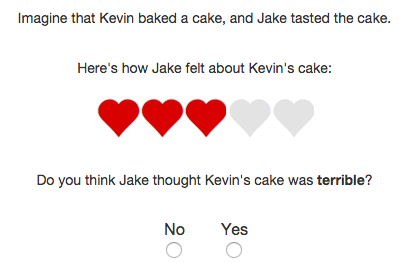
\includegraphics[width=3.2in]{figures/example.png}
\caption{\label{fig:ex} Example of a trial in Experiment 1.}
\end{centering} 
\end{figure}

\section{Experiment 1: Literal semantics}

%\ndg{briefly motivate this expt.}
Experiment 1 measured people's judgment for literal semantic meanings of words: 
does the literal meaning of a word aptly describe how someone performed?
Responses in this Experiment would be used to set expected literal meanings of words in our formal model.

\subsection{Method}

\subsubsection{Participants}

30 participants with IP addresses in the United States were recruited on Amazon's Mechanical Turk. 

\subsubsection{Stimuli and Design}

We created 13 different context items, in which a person (e.g., Ann) gave a performance of some kind, and another person (e.g., Bob) evaluated it. For example, in one of the contexts, Ann baked a cake, and Bob tasted it. Bob's feelings toward Ann's cake (``\emph{true state}'') were shown on a scale out of five hearts (e.g., two out of five hearts filled in red color). The question of interest was ``Do you think Bob thought Ann's cake was X?'' where X could be one of five possible words: \emph{terrible}, \emph{bad}, \emph{okay}, \emph{good}, and \emph{amazing}. Each participant read 25 scenarios, depicting every possible combination of 5 true states and 5 words.The order of context items was randomized, and there were a maximum of two repeats of each context item per participant.

\subsubsection{Procedure}

Participants read scenarios and indicate their answer to each question by answering `No' or `Yes' (see Fig. \ref{fig:ex} for a screenshot of an example trial).\footnote{Link to Experiment 1: \url{http://langcog.stanford.edu/expts/EJY/polgrice/L2_J/polgrice_L2_J.html}} 

\subsection{Results}

%\ndg{this paragraph is kind of awkward, and too wordy. basically: the meanings were as you'd expect. see figure...}

Meanings of the words were as one would expect (see Figure \ref{fig:exp1}). 
Proportion of acceptances for a word given the true state peaked where the degree of positivity, neutrality and negativity of the state matched that of the word. 

\section{Experiment 2: True state inference}

Experiment 1 results were used as the literal meanings of utterances $W$ with respect to states $S$ --- the term $\denote{w}(s)$ in Eq. \ref{eq:L0}.
In Experiment 2, we examined listeners' inferences about the likely state of the world $s$ given a speaker's utterance (e.g. \emph{It was good.}) and a description of the speaker's intentions (e.g. the speaker ``wanted to be nice'').

\subsection{Method}

\subsubsection{Participants}

35 participants with IP addresses in the United States were recruited on Amazon's Mechanical Turk. 

\subsubsection{Stimuli and Design}

The structure of the stimuli was the same as Experiment 2, except that, instead of providing information on the speaker (e.g., Bob)'s utterance and feelings about a person (e.g., Ann)'s performance (\emph{true state}) and asking for inference on Bob's goals, we provided information on Bob's utterance and his \emph{goal} and asked for participants' inference on the true state (i.e., Bob's true feelings about Ann's performance).

\subsubsection{Procedure}
Participants read each story (e.g., Ann baked a cake and asked Bob about it) followed by a prompt that said, 
e.g., ``Bob wanted to be nice: ``It was okay,'' he said.''
Then a question asked, ``How do you think Bob actually felt about Ann's cake?''
Participants indicated their answer on a scale of five hearts.

\subsection{Behavioral results}

%\ndg{same comment: too wordy.}

\begin{table}[t]
\caption{\label{tab:lmer2}  Coefficient estimates from a mixed-effects model predicting state inferences in Experiment 3.} 
\begin{center} 
\begin{tabular}{l r r r l} 
\hline
Predictor  &  Value (SE) & \emph{t}-value\\
\hline
Intercept (Honesty goal)  & 1.4 (.16) & 8.91 \\
Utterance & .41 (.05) &  8.58 \\
Niceness goal  & 1.9 (.19) & 10.2 \\
Meanness goal & .75 (.19) & 4.03 \\
Utterance $\times$ Niceness goal & -.69 (.05) & -13.5 \\
Utterance $\times$ Meanness goal & -.11 (.05) & -2.15 \\
\hline
\end{tabular} 
\end{center} 
\end{table}

Inferences of the actual rating for listener's performance, or the true state, varied depending on speaker's goal and utterance (Figure \ref{fig:exp3}).
\ndg{fig 3 is showing the mean heart rating and expected state? do we ever analyze the distribution over states?}
We fit a linear mixed-effects model\footnote{with the maximal convergent random effects structure: true state ~ goal $\times$ utterance + (utterance $|$ participant)} to look at the effects of information on speaker's goal and utterance on inferred true states, and found significant main effects for and interactions between utterance and goal. 

Given the speaker's goal to be honest, as predicted from the literal semantics distribution, inferred state positivity was correlated with utterance positivity: e.g., ``terrible'' implied approximately the true state of 1, ``amazing'' the state of 5. %Interestingly, state inferred based on the utterance ``[It was] bad'' was not judged to be different from the inferred state based on ``terrible,'' which is seemingly more negatively-connoted. In contrast, the inferred state based on ``good'' was less positive than inferred based on ``amazing.'' This may suggest that saying even a weakly negative remark (e.g., ``bad'') is face-threatening to a similar degree as making a more strongly negative comment, given that the speaker has already decided to express criticism. \ndg{?}
Given the speaker's goal to be nice, the inferred state positivity also increased with the utterance positivity, but participants inferred that the states are less positive compared to states given honesty goal, based on neutral and positive utterances. Based on the utterance ``amazing,'' participants inferred the true state to be close to 5 given the honesty goal, but they inferred the state to be around 3 given the niceness goal. This suggests that participants thought a speaker who was trying to be nice produced an utterance  with a literal meaning that is more positive that the speaker's true feelings toward the listener's performance.
Given the speaker's goal to be mean, participants inferred that the true states were more positive if the speaker's utterance was negative or neutral. 
But interestingly, if a positive utterance was produced with the goal to be mean, the true state was inferred to be worse compared to the states based on honesty and niceness goal. 
This response pattern might be due to people's attribution of sarcasm or irony to the speaker with meanness goal (see Discussion).

It should be noted that more positive utterances lead to inference of more positive states given the goal to be nice, which indicates that people think a ``nice'' speaker is still being somewhat informative with respect to communicating what the true state is. Thus, a nice speaker probably used the word ``amazing'' to describe an okay presentation rather than a terrible one.

\begin{figure}
\begin{centering} 
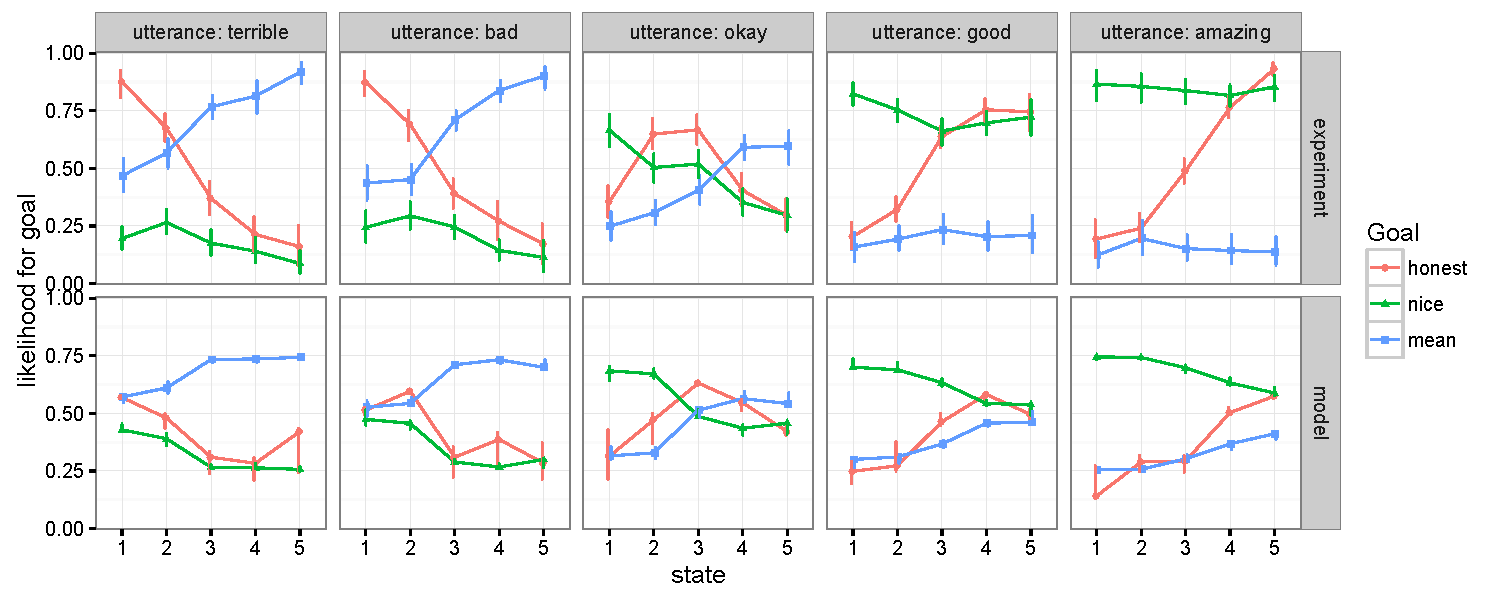
\includegraphics[width=3.2in]{figures/exp3.pdf}
\caption{\label{fig:exp3} Results from Experiment 3 (top) and model predictions (bottom). Average states inferred based on speaker's goal and utterance. Error bars represent 95\% confidence intervals.}
\end{centering} 
\end{figure}



%In addition, in each model, we include an explicit submodel of random guessing behavior, and model the behavioral data as mixture of this noise and the predictions of the pragmatic listener model $L_1$ (Eq.~\ref{eq:L1}).
%Including such a contamination parameter is important for getting reliable estimates of the parameters of the RSA model, which would otherwise be corrupted by this noise \cite{LW2014}. 
%We put a uniform prior over this mixture parameter $\phi \sim \text{Uniform}(0,1)$. 
%This mixture parameter provides an additional measure of goodness of fit: It shows the proportion of the data that is better explained by the cognitive model than by a model of random guessing. 

\subsection{Model predictions}

In this experiment, participants were told the speaker said $w$ as well as described what the speakers intentions were (e.g. \emph{Bob wanted to be nice}). 
To model this, we assume that the intentions (e.g. \emph{wanted to be nice}) modified the listener's prior distribution over goal-weights for the relevant goal. For example, if a speaker was trying to be nice, we interpret that to mean the speaker has a non-uniform prior distribution over $\beta_{nice}$ (in particular, we expect $\beta_{nice}$ to be skewed toward higher-values). 
We assume $\beta \sim \text{Beta}(\gamma, \delta)$, and for each goal condition (trying to be \emph{nice, mean, honest}), we put uninformative hyperpriors over the associated goal prior\footnote{For ease of interpretation, we are parametrizing the $\beta$ distribution by its mean and concentration. To recover the canonical shape parametrization, use $\gamma \delta$ and $(1-\gamma)\delta$.}.

%
\begin{eqnarray*}
& \gamma \sim  \text{Uniform}(0,1)\\
& \delta  \sim  \text{Uniform}(0, 20)
\end{eqnarray*}
For the unassociated goal priors (e.g. $\beta_{mean}$ and $\beta_{honest}$ when \emph{trying to be nice}), we use the same uniform priors we used to model the goal inference data.
\ndg{clarify what unassociated goal priors are...}

\begin{table}[]
\centering
\begin{tabular}{lll}
\hline
Expt. Condition  & Goal weight Mean & Concentration \\ \hline
(trying to be) Honest                        &   0.98 [0.86, 0.99]   & 18.8 [6.2, 19.9] \\
(trying to be) Nice                          & 0.99 [0.84, 1.0] & 19.0 [7.6, 20] \\
(trying to be) Mean                          &0.37 [0.01, 0.85] & 0.1[0.03, 2.1] \\ \hline
\end{tabular}
\caption{\label{tab:params} Inferred hyper-parameter values for Goal Priors in State Inference task.
For each experimental condition (trying to be X), we inferred the likely priors on the goal weights for the associated goal.
Values shown are MAP estimates and 95\% HDI for the parameter values.}
\end{table}
We ran 2 MCMC chains for 20,000 iterations, discarding the first 10,000 for burnin.
The MAP and 95\% HDI for $\lambda$ is 1.5 [1.2, 1.9]; for $\alpha$ is 2.4 [1.9, 3.0]. %; for $\phi$ is \red{0.09 [0.06, 0.13]}.
Inferred parameter values for the goal priors are shown in Table \ref{tab:params}.
\ndg{it'd be nicer to see this as a figure showing posterior predictives of the relevant beta's for each goal...}

The predictions of the model are shown in Figure \ref{fig:exp3}.
The model's expected posterior over states when the speaker is trying to be \emph{honest} increase as a function of the utterances likely of matching positive states (i.e. \emph{amazing} means a very high state).
When the model knows the speaker was trying to be \emph{nice}, the listener is more conservative in how it interprets positive utterances, with the difference between an honest utterance and a nice utterance increasing as the utterance becomes more likely to signal a higher valued state. 
For example, the difference between a ``nice'' \emph{amazing} and an ``honest'' \emph{amazing} is greater than the difference between a ``nice'' \emph{okay} and an ``honest'' \emph{okay}.
Inferences when the speaker is trying to be ``mean'' display the associated opposite behavior when the utterance is indeed negative (e.g. \emph{terrible}).
 %\mht{Describe model predictions.}
Overall, the model explains a lot the variance in the data $r^2(15) = 0.73$. 
The main discrepancies are with the goal ``trying to be mean'', as noted above (see Discussion). 
Among the other 2 goal conditions, the model explains almost all of the variance $r^2(10) = 0.94$. 

\subsection{Discussion}

The model captured key aspects of our empirical findings, albeit with some discrepancies.
Unlike the model predictions that the inferred states given honesty goal would be more positive throughout,
empirically, inferred states based on honesty and niceness goals did not differ from each other given negative utterances (``terrible'' and ``bad''), 
This may actually indicate a link between the two utilities we posited: 
``bad'' is a negative utterance, which suggests it was impossible for the speaker to be ``nice'' and satisfy the social utility, to save the listener's face. 
But a speaker who tried to cooperate with the listener by being nice would also want to cooperate in another sense, by being honest and satisfying the epistemic utility.  
Thus, participants might have reasoned that the speaker encountered an impossible situation to be cooperative with niceness and instead decided to cooperate with honesty. 

Also, people thought that a mean speaker saying ``[your cake] was amazing'' meant the true state was bad, which was in contrast to our model predictions. 
This may be due to irony in play: making an extremely positive remark about an extremely bad performance is perceived to be sarcastic and ill-intentioned \cite{colston1997}. 
Our model does not capture the sarcastic interpretation of a mean speaker who says \emph{It was amazing}; 
other RSA models have captured irony \cite{Kao2015}, and future work could combine the two extensions.

\ndg{it's also interesting that the model under-predicts the state for "amazing"/nice. perhaps this is because the params are adjusted to try to squash the mean state? what happens if we run the BDA leaving out meanness?
for the decrease in "amazing"/mean compared to "ok"/mean... could it just be a prior? eg maybe amazing performances are simply less likely? though that doesn't actually explain why a mean speaker would ever bother saying "amazing". so, yeah, probably need irony/snarkiness to explain this.}

\section{Experiment 3: Goal inference}

\begin{figure*}[t]
\begin{center} 
  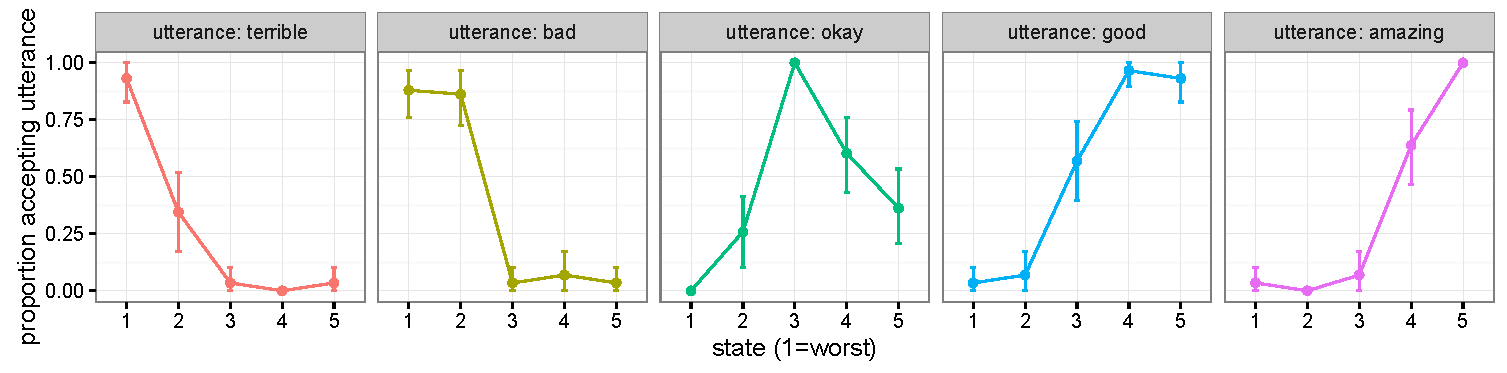
\includegraphics[width=.9\textwidth]{figures/exp1.pdf}
  \caption{\label{fig:exp1} Results from Experiment 1. Proportion of acceptances of words (shown in different colors) given the true state represented on a scale of hearts. Error bars represent 95\% confidence intervals.}
  \end{center} 
\end{figure*}

Experiment 3 probed listeners' inferences of the speaker's goals, given an utterance (e.g. \emph{``It was good''}) and a true state (e.g. 2 out of 5 hearts). 

\subsection{Method} 

\subsubsection{Participants}

45 participants with IP addresses in the United States were recruited on Amazon's Mechanical Turk. 

\subsubsection{Stimuli and Design}

We designed scenarios in which a person (e.g., Ann) gave some performance and asked for another person (e.g., Bob)'s opinion on the performance. The same context items and true states as Experiment 1 were used. Additionally, we provided information on what Bob actually said to Ann (e.g., ``It [your cake] was okay''), where Bob used one of the five possible words,  \emph{terrible}, \emph{bad}, \emph{okay}, \emph{good}, and \emph{amazing}. Then we asked participants to infer the likelihood of Bob's goals to be honest, nice, and mean. As in Experiment 1, each participant read 25 scenarios, depicting every possible combination of 5 true states and 5 words.The order of context items was randomized, and there were a maximum of two repeats of each context item per participant.

\subsubsection{Procedure}
Participants read each scenario followed by a question that read, ``Based on what Bob said, how likely do you think that Bob's goal was to be: honest; nice; mean,'' with the three goals placed in a random order below three slider bars, on which the participant could indicate each goal's likelihood.

\begin{figure*}[t]
\begin{center} 
  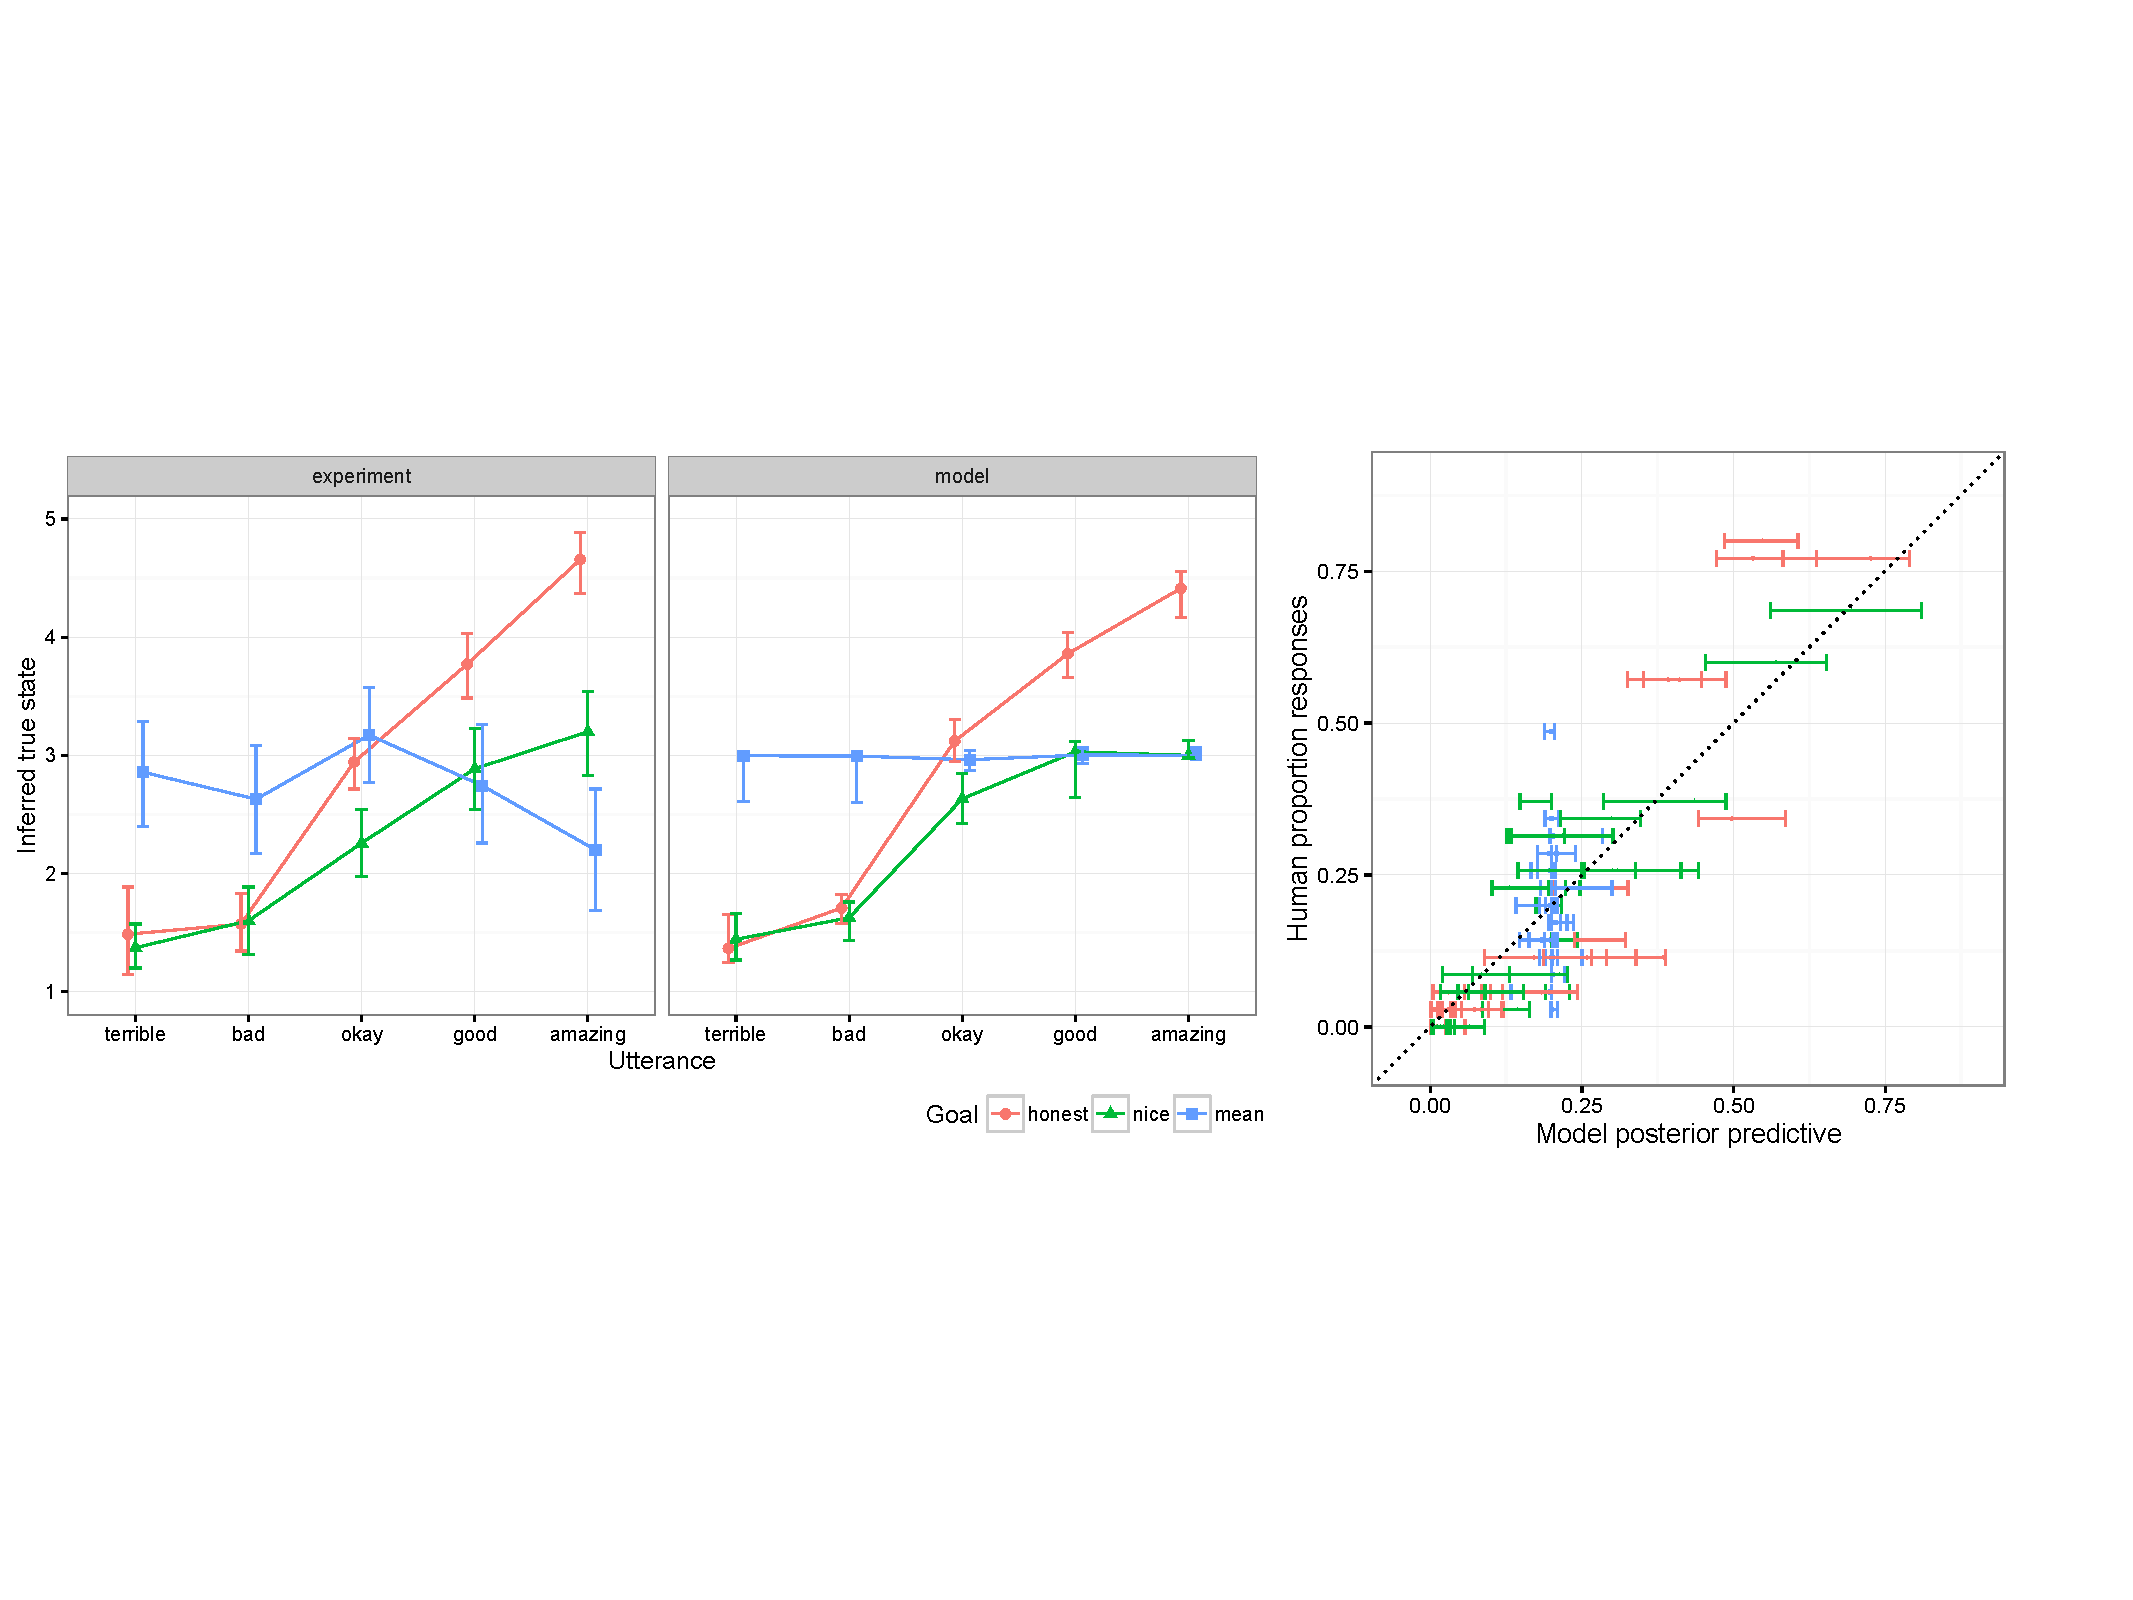
\includegraphics[width=.9\textwidth]{figures/exp2.pdf}
  \caption{\label{fig:exp2} Results from Experiment 2 (top) and model predictions (bottom). Attribution of speaker's goals (honest vs. nice vs. mean, shown in different colors) based on the true state and utterance. Error bars represent 95\% confidence intervals.}
  \end{center} 
\end{figure*}

\subsection{Behavioral results}

\begin{table}[t]
\caption{\label{tab:lmer1}  Coefficient estimates from mixed-effects models predicting goal attributions in Experiment 2.} 
\begin{center} 
\begin{tabular}{l r r r l} 
\hline
Predictor  &  Value (SE) & \emph{t}-value\\
\hline
\emph{Goal to be honest} \\
Intercept  & 1.5 (.04) & 34.1 \\
True state & -.35 (.01) &  -29.9 \\
Utterance & -.32 (.01) & -26.6 \\
True state $\times$ Utterance & .11 (.003) & 31.9 \\
\emph{Goal to be nice} \\
Intercept  & .07 (.04) & 1.70\\
True state & -.05 (.01) &  -5.46 \\
Utterance & .17 (.01) & 12.7 \\
True state $\times$ Utterance & .01 (.002) & 2.73 \\
\emph{Goal to be mean} \\ 
Intercept  & .37 (.04) & 9.18 \\
True state & .18 (.01) &  18.3 \\
Utterance & -.05 (.01) & -3.76 \\
True state $\times$ Utterance & -.04 (.003) & -12.2 \\
\hline
\end{tabular} 
\end{center} 
\end{table}

%\ndg{this section feels too wordy to me. don't need to describe what people can see in the figure, only need to point out aspects that are theoretically important or puzzling.}

Participants attributed likelihoods for speaker's goals differentially depending on the true state and utterance (see Figure \ref{fig:exp2}). We fit linear mixed-effects models\footnote{Models with the maximal convergent random effects structure: goal likelihood ~ true state $\times$ utterance + (utterance $|$ participant)} to measure the effects of true state and utterance (as numeric variables, ordered from the worst to the best) on the attribution of each goal (Table \ref{tab:lmer1}) and we found significant main effects and interactions of true state and utterance on each of the three goal attributions, though with varying effect sizes. 

For the honesty goal, the peak in the likelihood of honesty goal attribution occurred when the literal meaning of the utterance was close to the true state, based on the literal semantics distribution shown in Experiment 1. The honesty goal attribution was highly correlated with the literal semantics distribution given the state and utterance (r = 0.86). Attributions of niceness (``niceness goal'') generally showed slightly decreasing slope with improved true state given particular utterance (represented by each facet in Figure \ref{fig:exp2}). Attributions of meanness(``meanness goal'') showed the opposite pattern to niceness: its slope across different utterances generally increased as true state improved, indicating that un utterance is perceived to be more mean when the literal meaning is more negative than the actual state.

\subsection{Model predictions}

The model in Eq.~\ref{eq:L1} specifies a joint-belief distribution over the speaker's goals $\beta$ and possible states of the world $s$.
To compare to the empirical data, we condition on the true state of the world given in the experimental condition, and compare the marginal distribution of speaker's goals $\beta$ to the empirical ratings.
%In Experiment 2, participants were supplied with the ``true state'' $s$ as well as the speaker's utterance $w$, and were asked to rate the likely goals of the speaker. 
Here, we assume a uniform prior over the likely goals of the speaker, which is operationalized in the computational model as weights over the utilities: $\beta \sim \text{Uniform}(0,1)$ .

The computational model has 2 parameters: the speaker optimality parameter $\lambda$ in Eq.~\ref{eq:S1} and the value scale parameter $\alpha$ in the utility function. 
We put uninformative priors on these and infer their posterior credible values  via Bayesian data analysis.
\begin{eqnarray*}
& \lambda \sim \text{Uniform}(0,20)\\
& \alpha \sim \text{Uniform}(0, 5)
\end{eqnarray*}
We ran 2 MCMC chains for 40,000 iterations, discarding the first 20,000 for burnin.
The Maximum A-Posteriori (MAP) estimate and 95\% Highest Probability Density Interval (HDI) for $\lambda$ is 4.6 [4.0, 4.9]; for $\alpha$ is 1.17 [1.04, 1.31].%; for $\phi$ is 0.09 [0.06, 0.13].
%This is a relatively low value for $\phi$: The model explains about 90\% of the data set better than a model of random guessing.

%               Goal Parameter        MAP    credLow  credHigh
%             (fctr)    (fctr)      (dbl)      (dbl)     (dbl)
%1             alpha        NA 1.02553704 0.91319156 1.1865188
%2               phi        NA 0.08983868 0.05699245 0.1284084
%3 speakerOptimality        NA 6.81149016 5.76426562 7.8453595

%% sans guessing
%               Goal Parameter           MAP  credLow credHigh
%             (fctr)    (fctr)         (dbl)    (dbl)    (dbl)
%1             alpha        NA  1.1707125822 1.042176 1.311626
%2               phi        NA -0.0006369482 0.000000 0.000000
%3 speakerOptimality        NA  4.6635325286 4.033799 4.945555

To test what data the model actually predicts, we examine the posterior predictive distribution by marginalizing out the likely parameter values and generating predictions for what the data should look like, given our cognitive model and the inferred parameters.
The predictions of the model are shown in Figure \ref{fig:exp2} (bottom).
The model believes the speaker to be more honest when the utterance matches the true state of the world, as given by the literal semantics data (Figure \ref{fig:exp2}, red lines). 
Further, the model increases its ratings of niceness as the utterance better matches states with higher values (green bars, main effect of panel).
The goal to be mean displays the opposite behavior, decreasing as the utterance matches states with higher values (blue bars).
Overall, the model displays a strong quantitative fit to the goal inference data $r^2(75) = 0.87$.


\subsection{Discussion}

The model successfully captured the key patterns in the data: 
changing goal likelihoods based on the degree of match, and positivity/negativity bias of mismatch, between the utterance and true state. 

\ndg{say something about the biggest mismatches to the data? eg model seems to under-predict honesty?}

% asymmetry between niceness and meanness
There was an interesting asymmetry in the data between the niceness versus meanness goal attribution, 
when the true state and utterance were both very positive or very negative. 
For example, when the true state and utterance were both ``amazing,'' people's likelihood rating for niceness goal was at ceiling. 
However, when the true state and utterance were both ``terrible,'' people's rating for meanness goal was around 50\%. 
This perhaps reflects participants' expectation of a speaker to try to be kind and honest; 
speaker's critical remark (e.g., ``terrible'') is perceived to be out of a good will to be maximally truthful to the listener, 
rather than intention to damage the listener's reputation. 
\mht{Or is this a bias to expect speakers to be honest and nice, and when it is mean, it is explained away as honest?}.



\section{General Discussion}

%\ndg{start with the high level view: adding kindness goal to formal pragmatics model; data suggest that this is needed (how?) and that our model sort of explains it.}

Why would a speaker ever say something that is not maximally truthful? 
Communication is often looked at from the perspective successful transfer of information from speaker to hearer. 
Yet in the social realm, communication also can serve the social function of making the listener feel good, and thereby establishing a favorable social relationship between speaker and hearer.

In the current paper, we proposed that intuitively ``polite'' utterances arise from the want to be kind (i.e., save the listener's face), and an optimal speaker tries to balance the want to be kind and want to be informative, and produces utterances of varying degrees of politeness that reflect this balance.
To test this, we examined people's inferential judgment on a speaker's utterance addressing evaluation of the listener's performance. 
As we predicted, people inferred the rating that a performance actually deserves
differentially based on what the speaker said and whether the speaker's intended goal was to be honest, nice or mean. 
We also found that people attributed goals to speakers depending on 
how much the literal utterance meaning matches the actual rating the performance deserves (higher attribution for goal to be honest) 
and how much positive bias (goal to be nice) or negative bias (goal to be mean) the utterance meaning carries. 

We also extended the previous formal pragmatics models based on epistemic utility (i.e., information transfer)
and proposed an addition of social utility (i.e., face-saving).
This is the first work to generalize the Rational Speech-Act theory to include utility parameters not based on the successful transfer of information. 

Will machines ever be polite? 
Politeness requires more than merely saying conventionalized words (\emph{please}, \emph{thank you}) at the right moments; it requires a balance of informativity and kindness. 
Politeness does not deviate from rational communication,
it is rather what makes human communication rational, by serving a key social function of maintaining relationships.
The formal model presented in this work moves us closer to computation with tact, to communication with consideration.


% Include next steps here?
% How do inferential patterns change with situations that vary goals that speakers should prioritize?
% Is polite speakers' intention for listeners to know what their goals are? How does this (display of) intention depend  on the context as well?

\bibliographystyle{apacite}

\setlength{\bibleftmargin}{.125in}
\setlength{\bibindent}{-\bibleftmargin}

\bibliography{politeness}


\end{document}
